%!TEX root=../../main.tex
\section{Frontend}
\subsection{Theoretische Konzeption}
\cite{dont-kmake-me-think-usability}
\subsection{Visuelle Konzeption}
\begin{figure}[H]
	\centering
	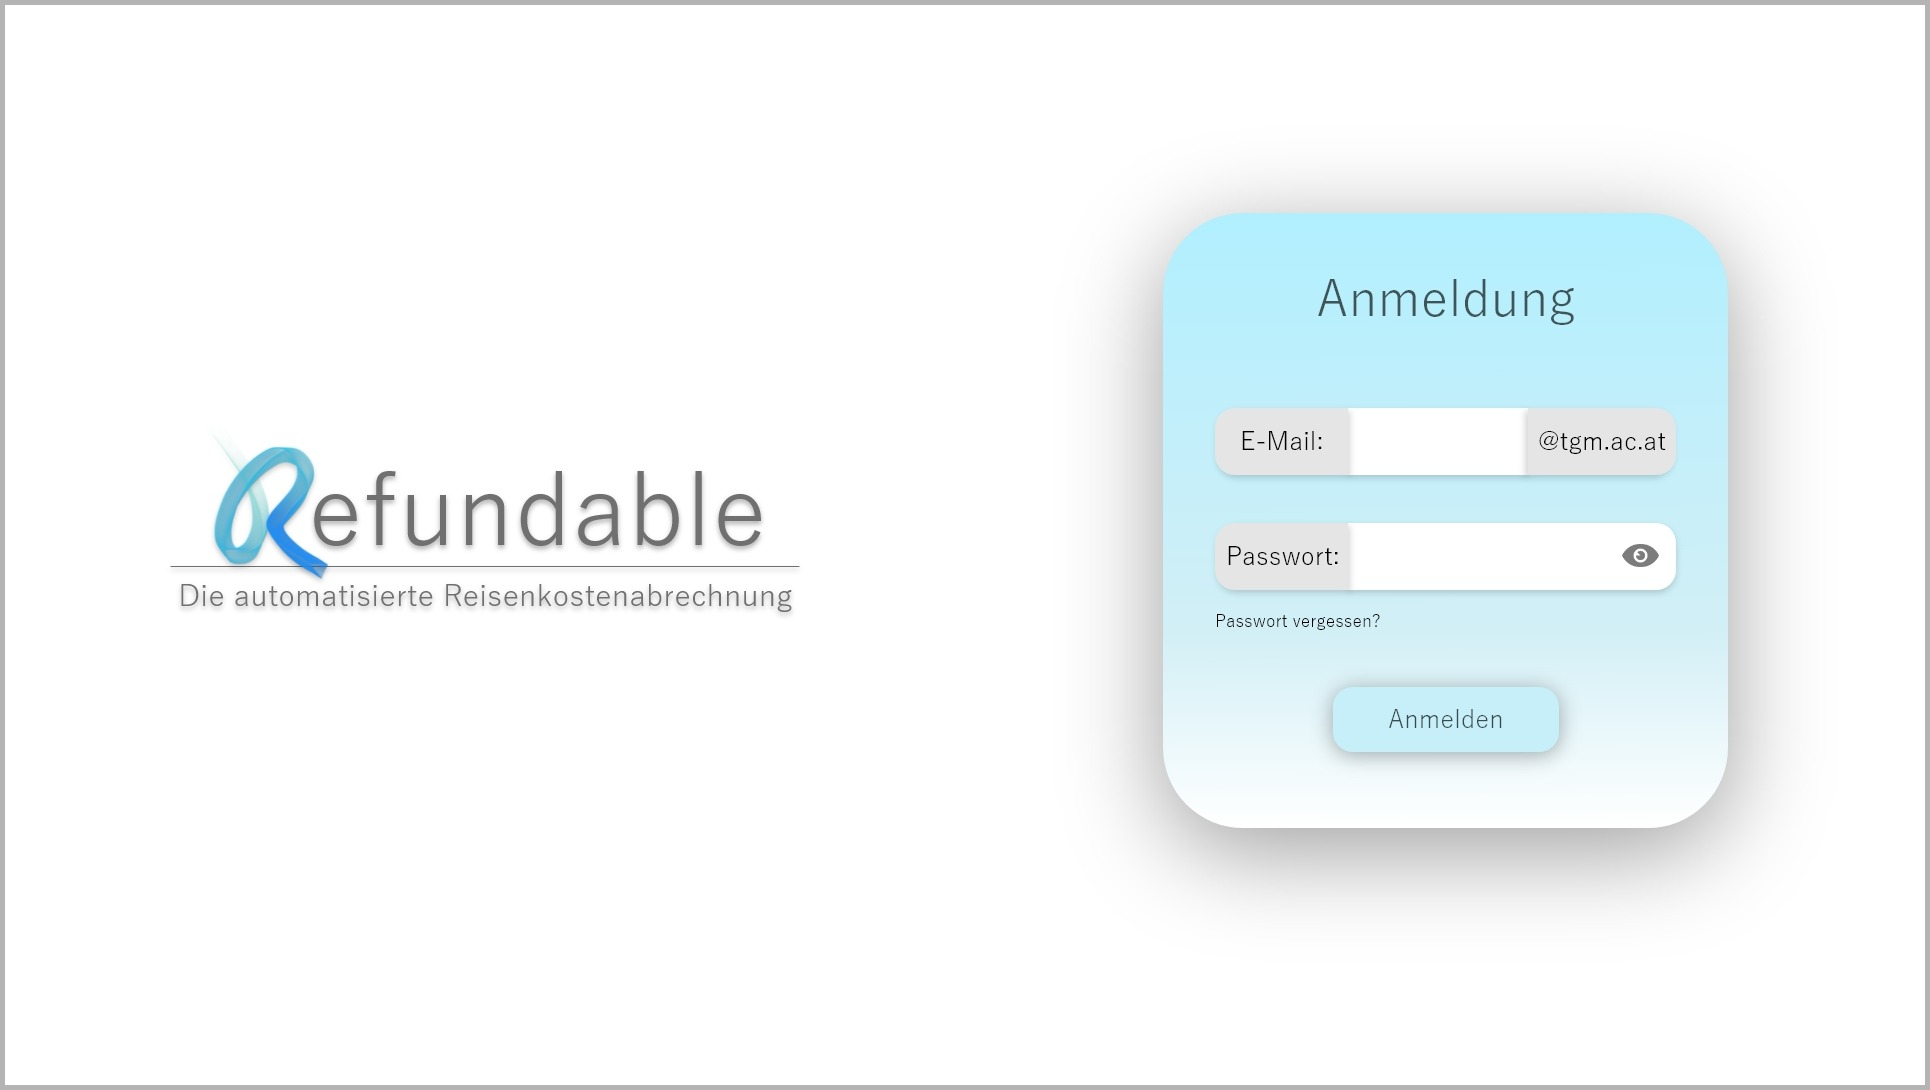
\includegraphics[width=1\linewidth]{images/Mockup-Startseite}
	\caption[Mockup Login]{Das Mockup der Login Seite}
	\label{fig:mockupLogin}
\end{figure}
\begin{figure}[H]
	\centering
	
\includegraphics[width=1\linewidth]{images/Mockup-Startseite-eingeloggt}
	\caption[Mockup Startseite]{Das Mockup der Startseite, nachdem man sich eingeloggt hat}
	\label{fig:mockupStart}
\end{figure}
\begin{figure}[H]
	\centering
	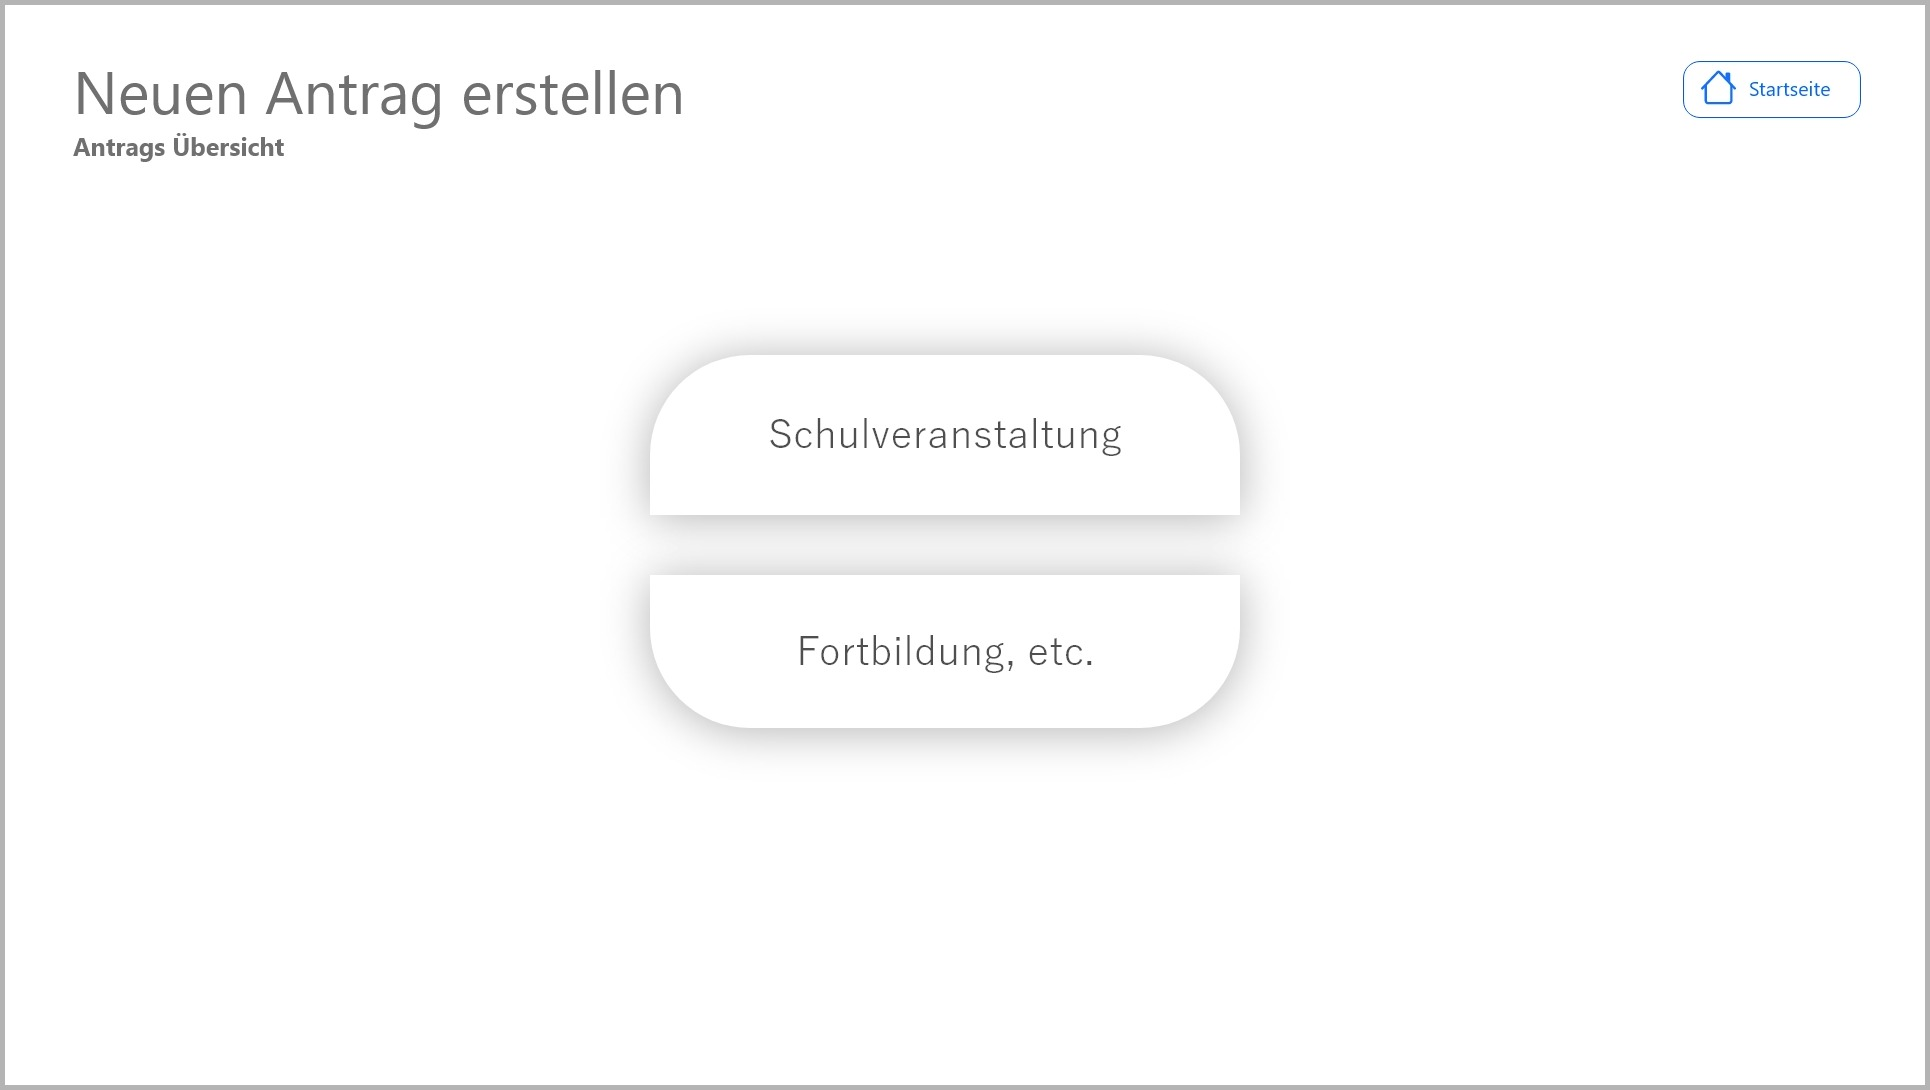
\includegraphics[width=1\linewidth]{images/Mockup-Neuer-Antrag}
	\caption[Mockup neuer Antrag]{Das Mockup der Seite, auf der man eine Antragsart auswählen kann}
	\label{fig:mockupNeu}
\end{figure}
\begin{figure}[H]
	\centering
	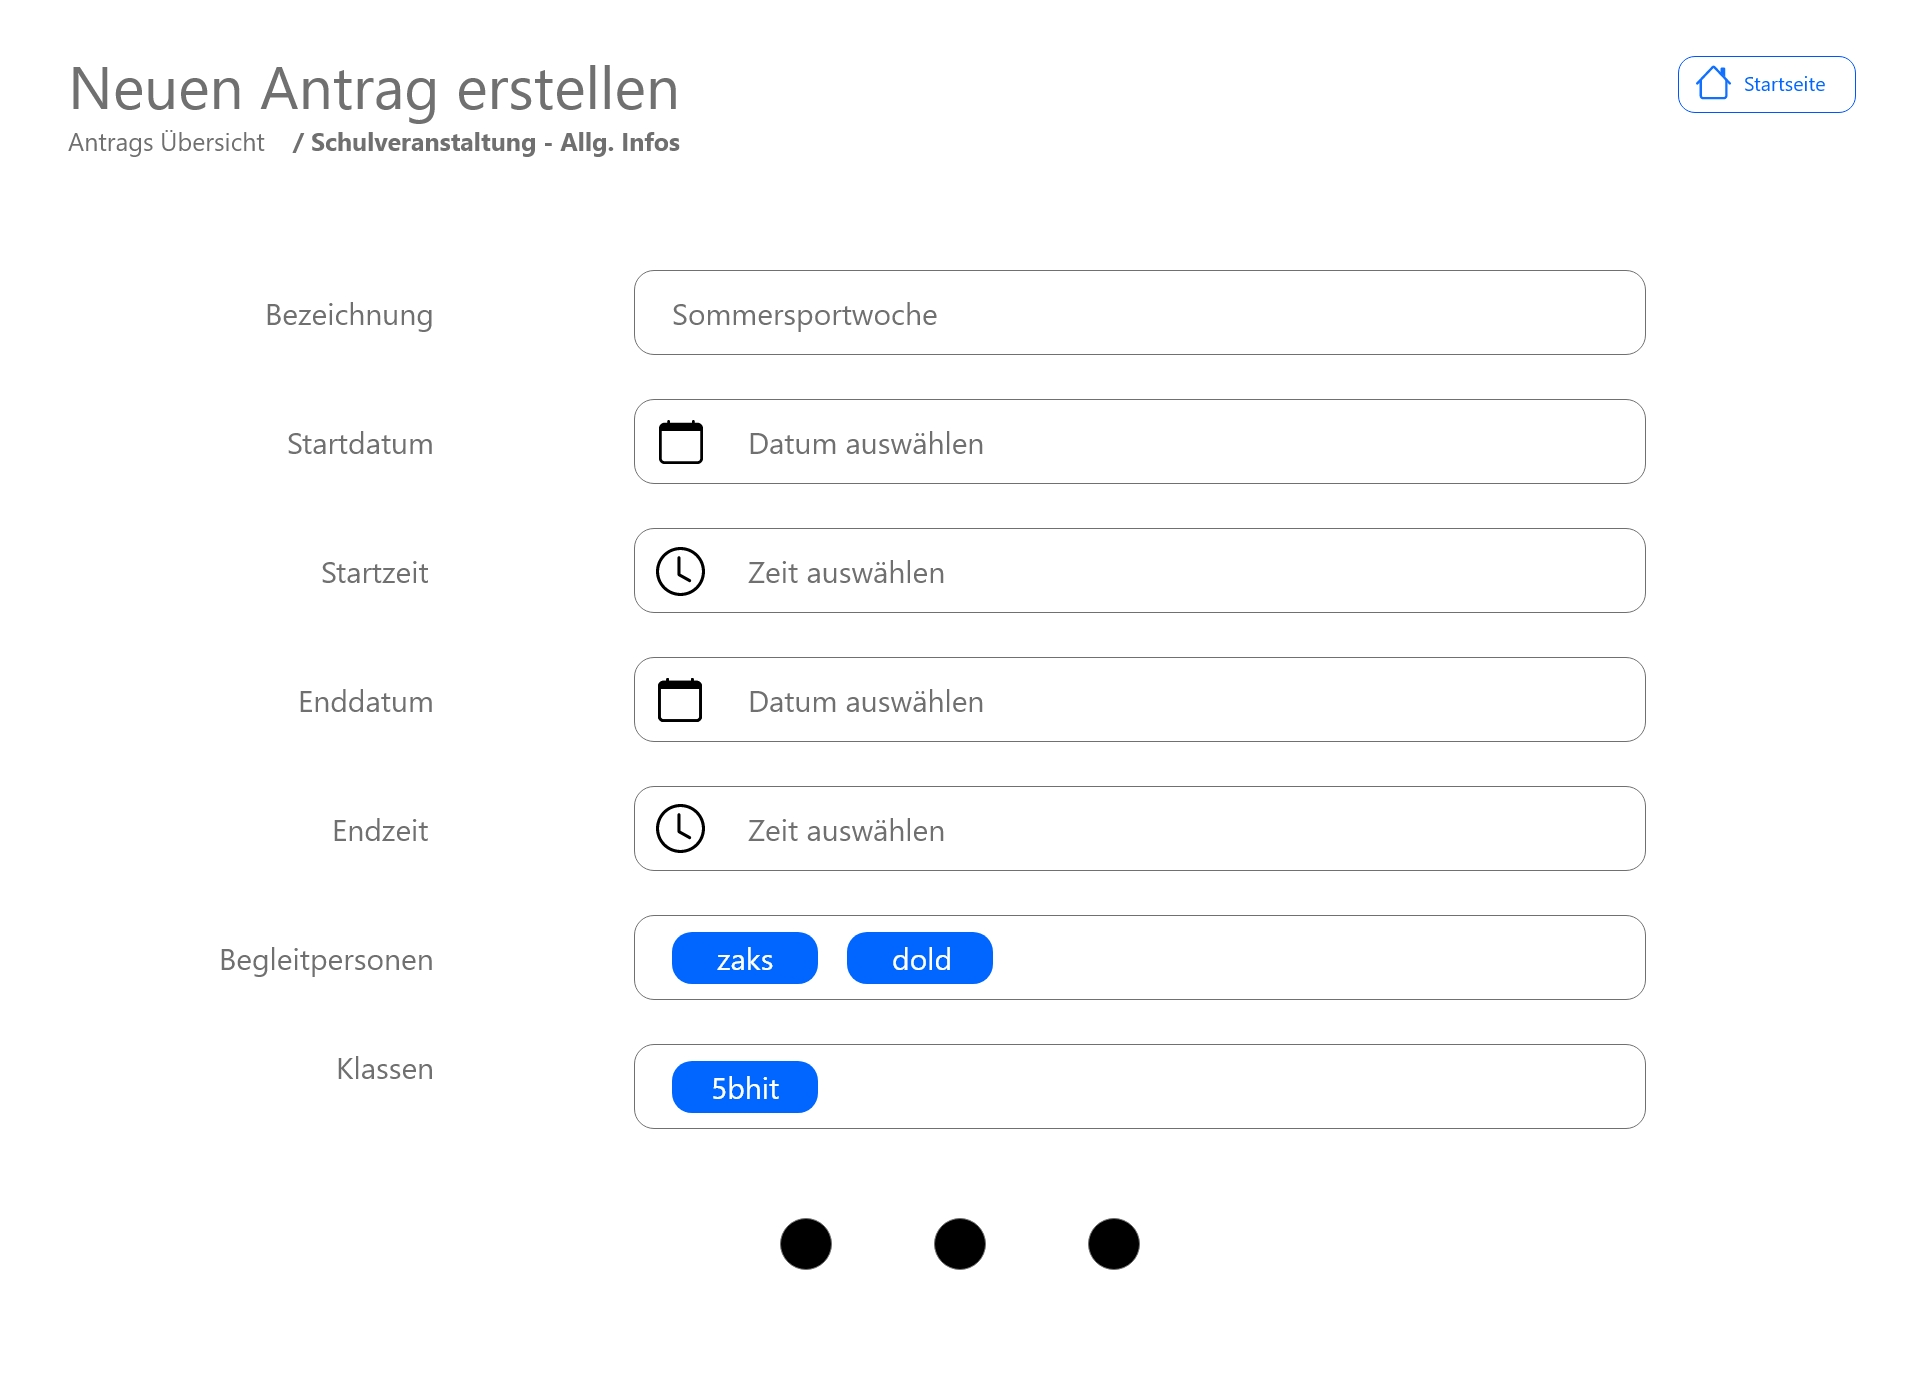
\includegraphics[width=1\linewidth]{images/Mockup-Antrag-erstellen}
	\caption[Mockup Antrag erstellen]{Das Mockup zum erstellen einer neuen Schulveranstaltung}
	\label{fig:mockupErstellen}
\end{figure}
\begin{figure}[H]
	\centering
	\includegraphics[width=1\linewidth]{images/Mockup-Alle-Anträge}
	\caption[Mockup Alle Anträge]{Das Mockup, welches alle Anträge einer gewissen Person veranschaulicht}
	\label{fig:mockupAlle}
\end{figure}
\begin{figure}[H]
	\centering
	\includegraphics[width=1\linewidth]{images/Mockup-Aktive-Anträge}
	\caption[Mokup aktive Anträge]{Das Mockup, welches alle aktiven Anträge einer gewissen Person veranschaulicht}
	\label{fig:mockupAktive}
\end{figure}
\begin{figure}[H]
	\centering
	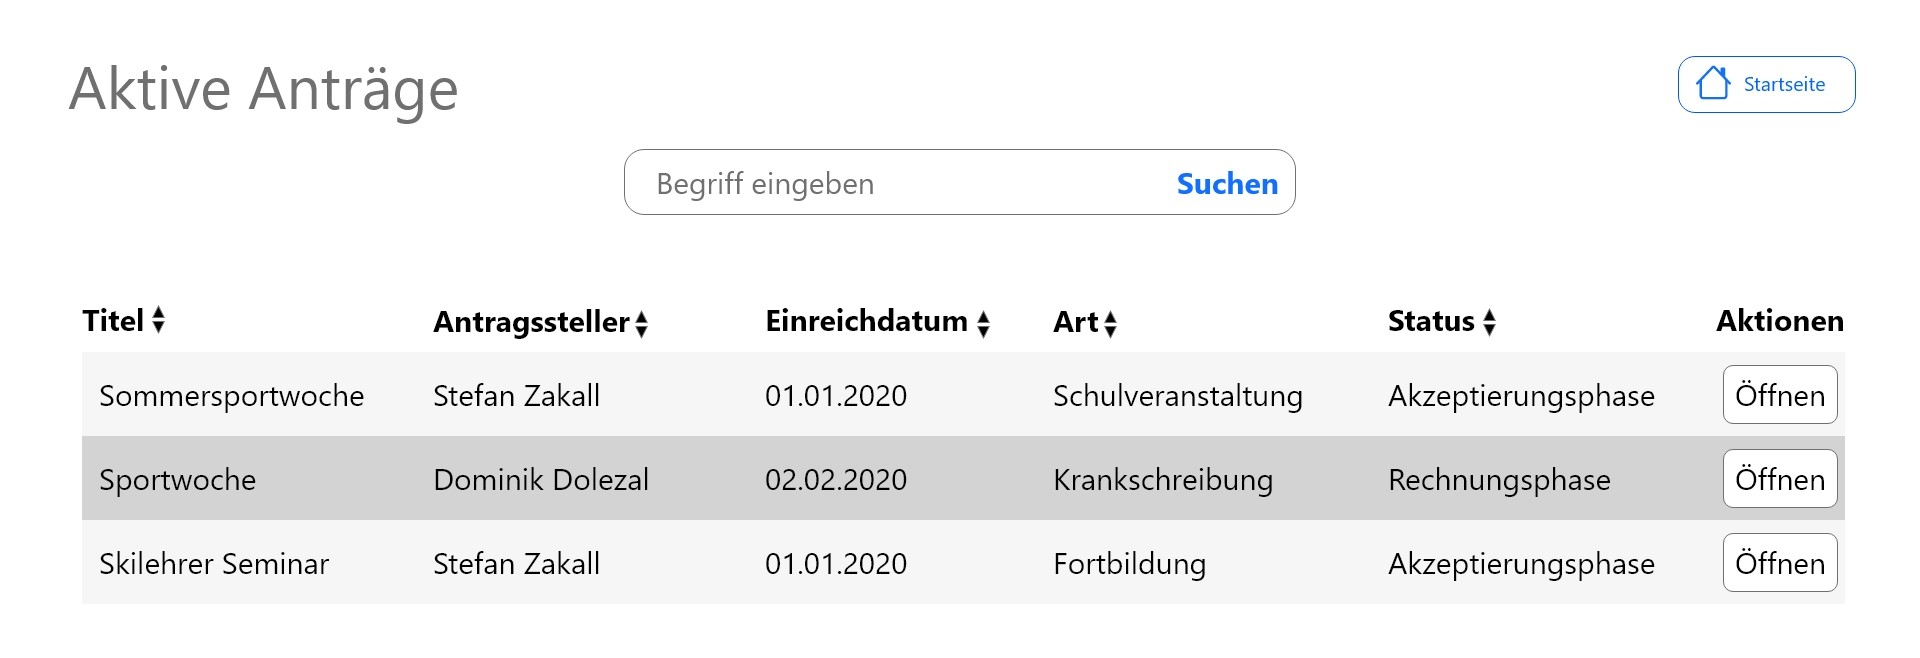
\includegraphics[width=1\linewidth]{images/Mockup-Admin}
	\caption[Mockup Adminansicht]{Das Mockup, der Admin Ansicht, zum akzeptieren und ablehnen von Anträgen}
	\label{fig:mockupAdmin}
\end{figure}
\begin{figure}[H]
	\centering
	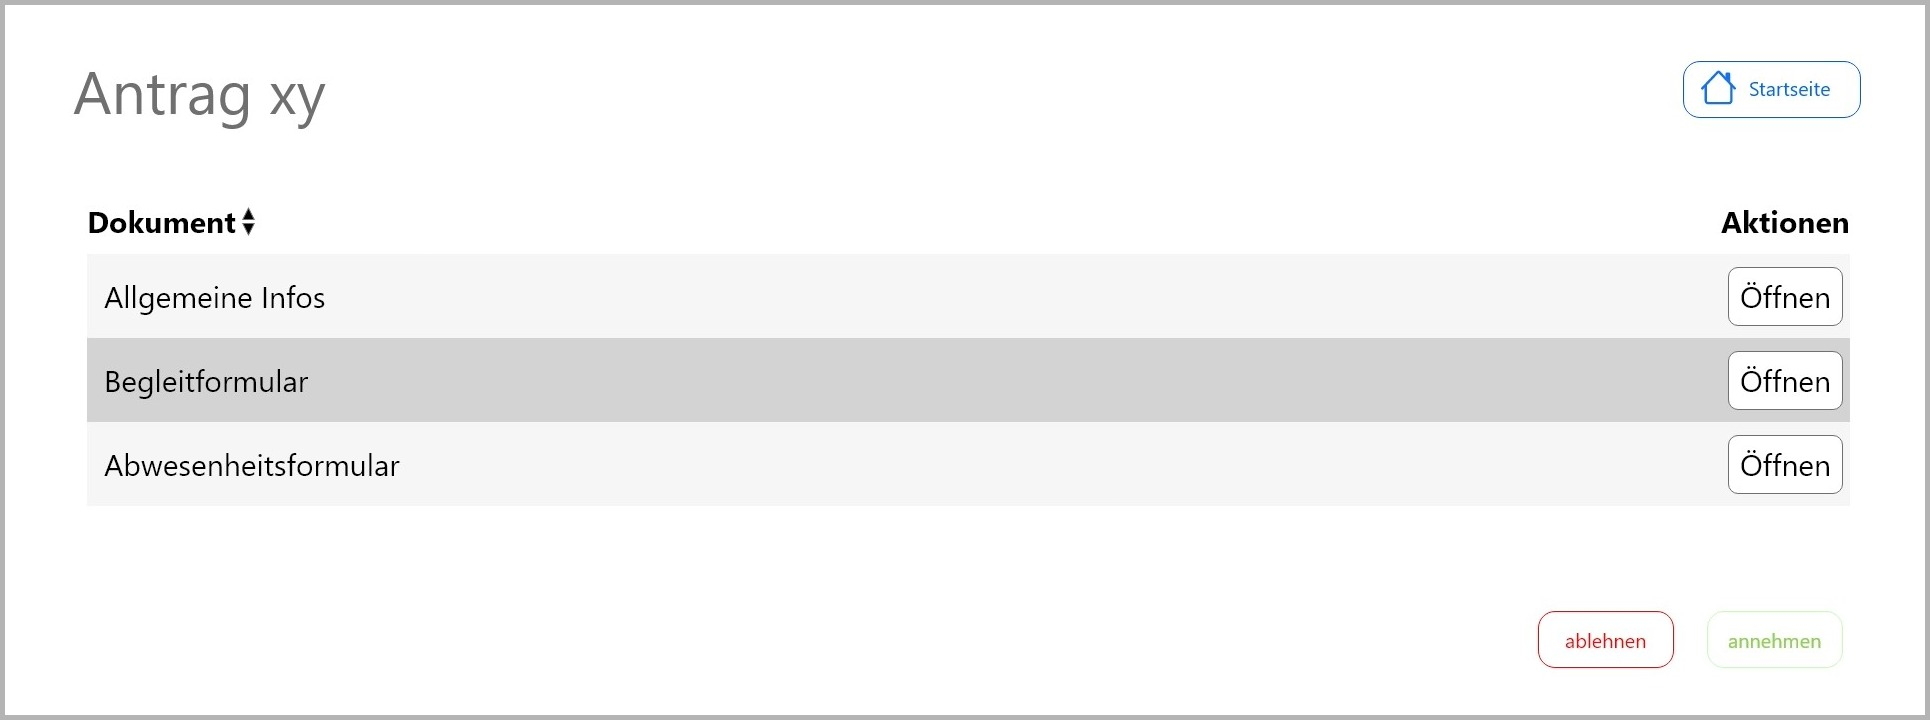
\includegraphics[width=1\linewidth]{images/Mockup-Antragsansicht}
	\caption[Mockup Antragsansicht]{Das Mockup, welches einen eingereichten Antrag veranschaulicht}
	\label{fig:mockupAntrag}
\end{figure}